\documentclass{article}
\usepackage[german]{babel}
\usepackage[utf8]{inputenc}

% References and Bibliography
\usepackage[hidelinks]{hyperref}
\usepackage[natbibapa]{apacite}
\usepackage{natbib}
\bibliographystyle{apacite}

% align for equations
\usepackage{amsfonts}
\usepackage{mathtools}

% Table formatting
\usepackage{booktabs}

% Code blocks for Python
\usepackage{listings}
\usepackage{color}
\usepackage{inconsolata}

\definecolor{codegreen}{rgb}{0,0.6,0}
\definecolor{codegray}{rgb}{0.5,0.5,0.5}
\definecolor{codepurple}{rgb}{0.58,0,0.82}
\definecolor{backcolour}{rgb}{0.95,0.95,0.92}

\lstdefinestyle{CustomPython}{
	backgroundcolor=\color{backcolour},   
	commentstyle=\color{codegreen},
	keywordstyle=\color{magenta},
	numberstyle=\tiny\color{codegray},
	stringstyle=\color{codepurple},
	basicstyle=\footnotesize,
	breakatwhitespace=false,         
	breaklines=true,                 
	captionpos=b,                    
	keepspaces=true,                 
	numbers=left,                    
	numbersep=5pt,                  
	showspaces=false,                
	showstringspaces=false,
	showtabs=false,                  
	tabsize=2,
	basicstyle=\scriptsize\ttfamily
}

\lstset{style=CustomPython}

\newcommand{\documentlanguage}{english}  % Change to german if needed

\begin{document}
\begin{titlepage}
\begin{center}
	\vspace{3em}	
    {\Huge\bfseries Proseminar - \textit{Grundlagen des maschinellen Lernens}\par}
    \vspace{2em}
    {\huge \textit{PyTorch, TensorFlow und Keras} \par}
    \vspace{3em}
    Autor\\
	\vspace{1em}
    {\Large \textit{Pavel Zwerschke}\par}
    \vspace{1em}
    Matrikelnummer: \textit{2223263}\\
    \vspace{3em}
    Datum:\\
	\vspace{1em}
    Karlsruhe, \today
\end{center}
\end{titlepage}
\newpage
\setcounter{page}{1}
\pagenumbering{Roman}
\section*{Abstract | Zusammenfassung}
Über die Jahre hinweg gab es bereits viele verschiedene Frameworks für das Programmieren 
mit Algorithmen im Bereich maschinelles Lernen. Von diesen vielen Frameworks 
haben sich schlussendlich zwei Frameworks durchgesetzt, nämlich PyTorch und TensorFlow. 
In diesem Proseminar betrachten wir diese beiden Frameworks und gehen darauf ein, 
wie man mit diesen Multi Layer Perceptrons und Convolutional Neural Networks 
erstellen und trainieren kann und vergleichen die beiden Frameworks schlussendlich.
PyTorch, TensorFlow und Keras sind hervorragende Tools, mit denen man mit 
relativ wenig Aufwand neuronale Netze erstellen kann. Wenn man vorhat, sich 
mit Machine Learning zu beschäftigen, sollte man auf jeden Fall mit mindestens einem der 
Frameworks gut umgehen können.
\newpage
\tableofcontents
\newpage
\setcounter{page}{1}
\pagenumbering{arabic}
\section{Introduction | Einleitung}
Mandatory. Questions like: What is the topic of this work, what's the broader context (topic of the proseminar), why is it relevant?

\section{PyTorch}
\subsection{Daten laden und präparieren}

\lstinputlisting[label=py:load-data-pytorch, language=Python, caption=MNIST Datensatz mit TorchVision herunterladen.]{code/load-data-pytorch.py}

\subsection{Modellerstellung}

\lstinputlisting[label=py:load-data-pytorch, language=Python, caption=Modellerstellung in PyTorch.]{code/create-model-pytorch.py}

\subsection{Modell trainieren}

\lstinputlisting[label=py:load-data-pytorch, language=Python, caption=Modell trainieren in PyTorch.]{code/train-model-pytorch.py}

\section{TensorFlow und Keras}
\subsection{Daten laden und präparieren}

\lstinputlisting[label=py:load-data-pytorch, language=Python, caption=MNIST Datensatz mit \texttt{keras.datasets} herunterladen.]{code/load-data-tensorflow.py}

\subsection{Modellerstellung}

\lstinputlisting[label=py:load-data-pytorch, language=Python, caption=Modellerstellung in TensorFlow.]{code/create-model-tensorflow.py}

\subsection{Modell trainieren}

\lstinputlisting[label=py:load-data-pytorch, language=Python, caption=Modell trainieren in TensorFlow.]{code/train-model-tensorflow.py}

\section{Zusammenfassung und Fazit}
Mandatory. Short summary of the most important aspects of the report.
If possible: What are open challenges?

\newpage
\section{\LaTeX Examples}
As a help to get started with this template. To be deleted for submission.
\subsection{Citation examples}
\citet{campbell:2017} define the stages of information processing in a nervous system as: "sensory input, integration, and motor output". \\
The stages of information processing in a nervous system are defined as: "sensory input, integration, and motor output" \citep{campbell:2017}. 

\subsection{Table example}
\begin{table}[htbp]
    \centering
    \begin{tabular}{lrl}
    \toprule
    labels   & numbers & annotation \\
    \midrule
    abra     &  1.23   & \textbf{this is important}\\
    cadabra  &  2.34   & this isn't\\
    \bottomrule
    \end{tabular}
    \caption{Some random numbers}
    \label{tab:random}
\end{table}

\subsection{Figure examples}
This is a png file, it gets blurry when you zoom in:
\begin{figure}[htbp]
    \centering
    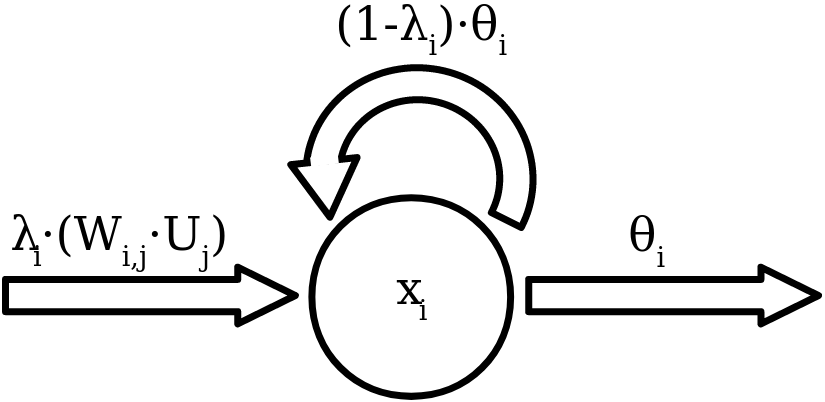
\includegraphics[width=.7\textwidth]{figures/leaky_integration.png}
    \caption{Symbolic representation of a leaky integrating neuron.}
    \label{fig:leaky_integration}
\end{figure}

This is an eps file, it is always sharp:\\
Notice how the formatting option "[htbp]" allows for the figure to be moved around to page \pageref{fig:activation_function}. Hence, it is best to rather write: The eps file in figure \ref{fig:activation_function} always stays sharp.
\begin{figure}[htbp]
    \centering
    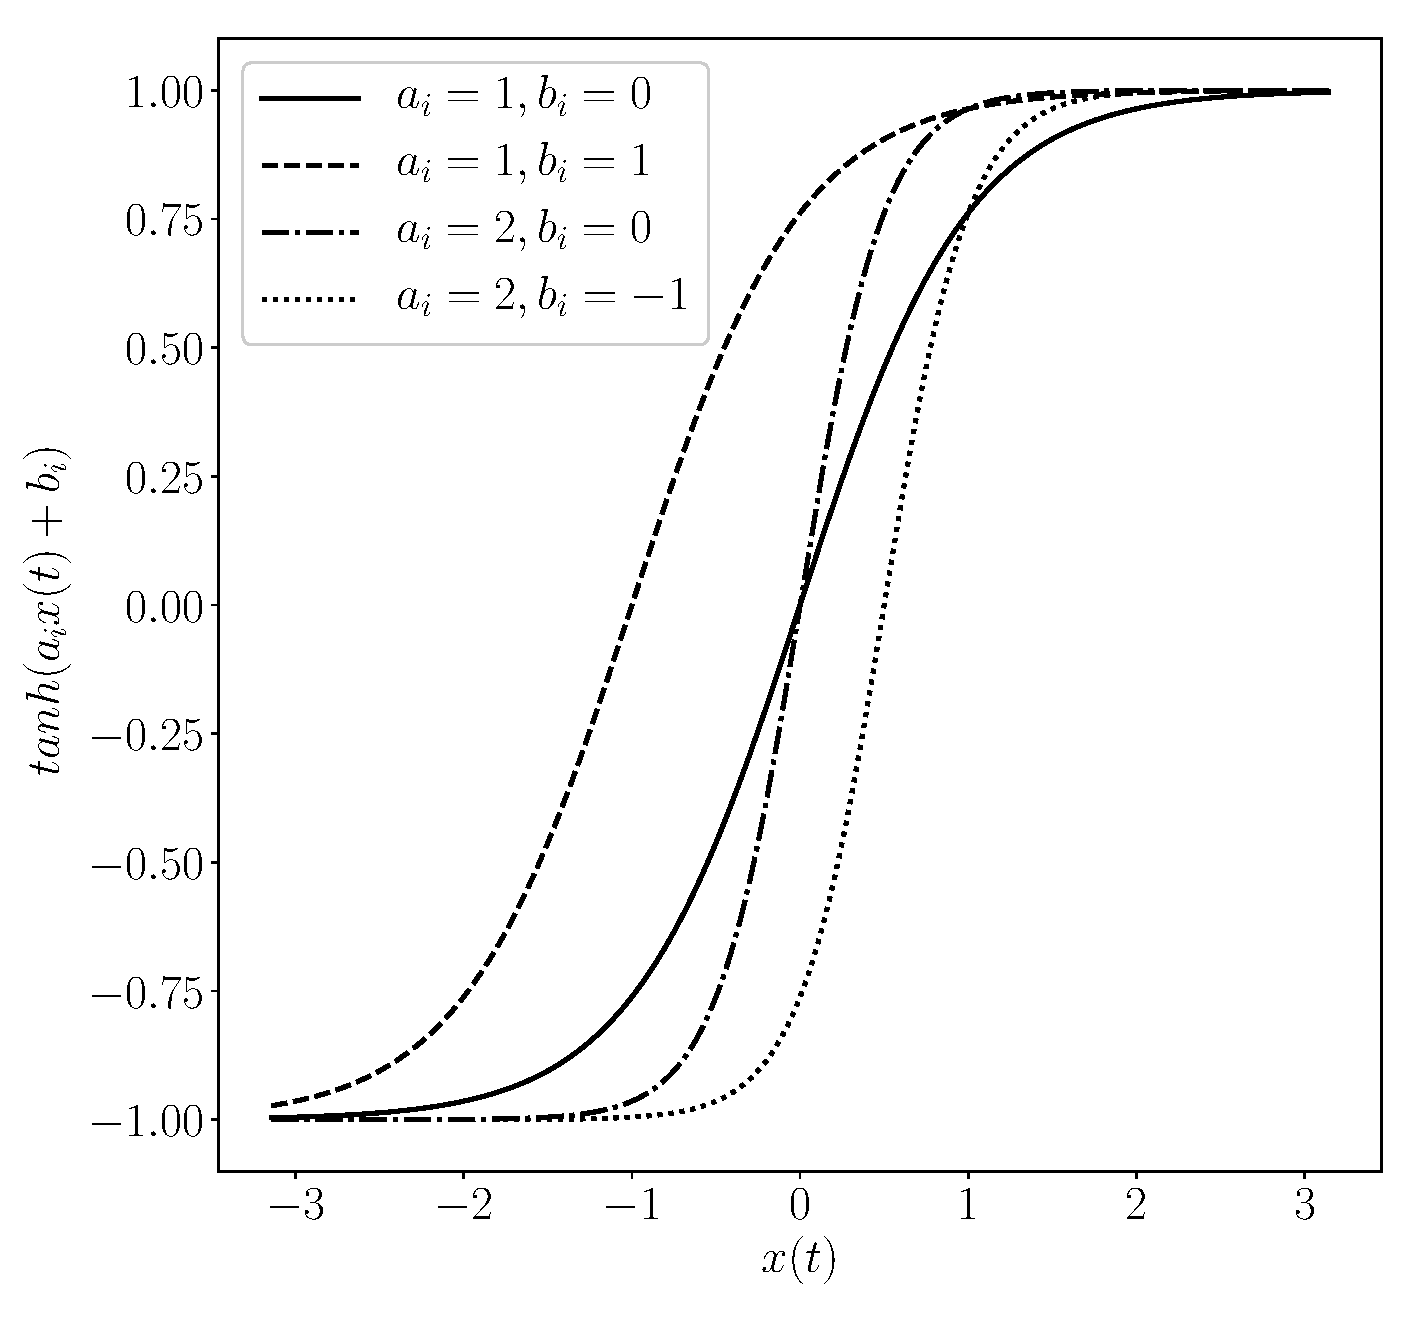
\includegraphics[width=.7\textwidth]{figures/activation_functions}
    \caption{Shapes of a parametrized tanh activation function.}
    \label{fig:activation_function}
\end{figure}

\subsection{Math example}
The state update of the leaky integrating neuron in figure \ref{fig:leaky_integration} can be formulated as:
\begin{align}
    x_i(t+1) &= \lambda_i \cdot \left(W_{i,j} \cdot U_j(t)\right) + (1-\lambda_i) \cdot \theta_i(t)
    \label{eq:leaky_integration}
\end{align}

\subsection{Footnote example}
The implementation is available on github\footnote{https://github.com/schniewmatz/recurrence}.
\newpage
\bibliography{bibliography}{}
\end{document}
